\subsection{Configurazione Collegamento al Server}\label{CCS}

Una volta aggiunto alla dashboard di \textit{Grafana} il pannello \textit{G\&B} per poter interagire in modo efficace con il pannello è necessaria, come prima operazione, configurare il collegamento al server, che è il componente che si occupa delle operazioni di ricalcolo delle probabilità. Tale operazione funge da precondizione per ogni altra funzionalità del prodotto.\\
Per poter effettuare l'operazione in esame l'utente deve innanzittuto accedere alla sezione \textbf{Server Settings} del menù di Edit del pannello, attraverso il percorso \textbf{Edit > Server Settings}.

\begin{figure}[H]
	\begin{center}
		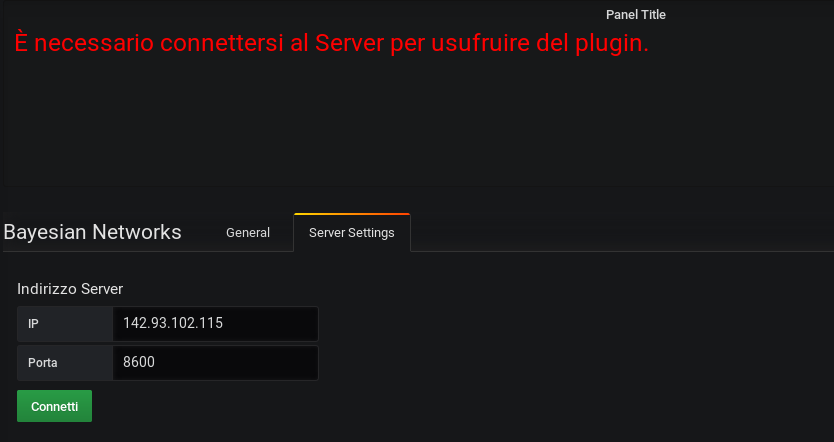
\includegraphics[scale=0.5]{./images/ServerSettings.png}
		 \caption{Sezione "Server Settings" del menù di Edit del Pannello \textit{G\&B}}	
		 \label{ServerSettings}
	\end{center}
\end{figure}

All'utente verrà dunque chiesto di inserire, negli appositi campi dati indicati in Figura \ref{ServerSettings}:
\begin{enumerate}
	\item \textbf{Indirizzo IP} del Server;
	\item \textbf{Porta} del Server in ascolto.
\end{enumerate}
Una volta editati i campi dati indicati l'utente deve confermare le proprie scelte premendo il pulsante \textbf{Connetti}.\\
Nel caso in cui il cui la configurazione del server sia andata a buon fine l'utente viene avvisato dell'avvenuto collegamento attraverso un messaggio di notifica (Figura \ref{NotificaServer}).

\begin{figure}[H]
	\begin{center}
		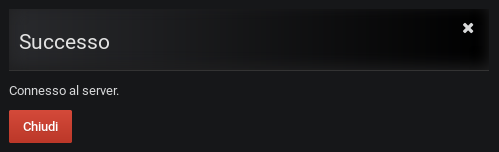
\includegraphics[scale=0.6]{./images/NotificaServer.png}
		 \caption{Notifica di avvenuto collegamento del Server}	
		 \label{NotificaServer}
	\end{center}
\end{figure}

~\\
\textbf{\textcolor{red}{ATTENZIONE}}: Nel caso in cui l'utente abbia commesso degli errori in fase di compilazione dei campi dati l'operazione non va a buon fine e l'utente viene avvisato degli errori commessi da un messaggio di errore (Figura \ref{ErroreServer}).

\begin{figure}[H]
	\begin{center}
		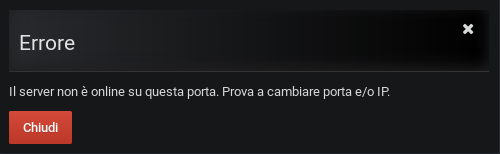
\includegraphics[scale=0.6]{./images/ErroreServer.png}
		 \caption{Messaggio di Errore configurazione Server}	
		 \label{ErroreServer}
	\end{center}
\end{figure}
